
%<<setup-child, include = FALSE>>=
%library(knitr)
%library(ggplot2)
%library(microbenchmark)
%set_parent("../style/preamble.Rnw")
%@

\input{../../2021/style/preamble4tex}
% dependencies: amsmath, amssymb, dsfont
% math spaces
\ifdefined\N
\renewcommand{\N}{\mathds{N}} % N, naturals
\else \newcommand{\N}{\mathds{N}} \fi
\newcommand{\Z}{\mathds{Z}} % Z, integers
\newcommand{\Q}{\mathds{Q}} % Q, rationals
\newcommand{\R}{\mathds{R}} % R, reals
\ifdefined\C
\renewcommand{\C}{\mathds{C}} % C, complex
\else \newcommand{\C}{\mathds{C}} \fi
\newcommand{\continuous}{\mathcal{C}} % C, space of continuous functions
\newcommand{\M}{\mathcal{M}} % machine numbers
\newcommand{\epsm}{\epsilon_m} % maximum error

% counting / finite sets
\newcommand{\setzo}{\{0, 1\}} % set 0, 1
\newcommand{\setmp}{\{-1, +1\}} % set -1, 1
\newcommand{\unitint}{[0, 1]} % unit interval

% basic math stuff
\newcommand{\xt}{\tilde x} % x tilde
\newcommand{\argmin}{\mathop{\mathrm{arg\,min}}} % argmin
\newcommand{\argmax}{\mathop{\mathrm{arg\,max}}} % argmax
\newcommand{\argminlim}{\argmin\limits} % argmin with limits
\newcommand{\argmaxlim}{\argmax\limits} % argmax with limits
\newcommand{\sign}{\operatorname{sign}} % sign, signum
\newcommand{\I}{\mathbb{I}} % I, indicator
\newcommand{\order}{\mathcal{O}} % O, order
\newcommand{\bigO}{\mathcal{O}} % Big-O Landau
\newcommand{\littleo}{{o}} % Little-o Landau
\newcommand{\pd}[2]{\frac{\partial{#1}}{\partial #2}} % partial derivative
\newcommand{\floorlr}[1]{\left\lfloor #1 \right\rfloor} % floor
\newcommand{\ceillr}[1]{\left\lceil #1 \right\rceil} % ceiling
\newcommand{\indep}{\perp \!\!\! \perp} % independence symbol

% sums and products
\newcommand{\sumin}{\sum\limits_{i=1}^n} % summation from i=1 to n
\newcommand{\sumim}{\sum\limits_{i=1}^m} % summation from i=1 to m
\newcommand{\sumjn}{\sum\limits_{j=1}^n} % summation from j=1 to p
\newcommand{\sumjp}{\sum\limits_{j=1}^p} % summation from j=1 to p
\newcommand{\sumik}{\sum\limits_{i=1}^k} % summation from i=1 to k
\newcommand{\sumkg}{\sum\limits_{k=1}^g} % summation from k=1 to g
\newcommand{\sumjg}{\sum\limits_{j=1}^g} % summation from j=1 to g
\newcommand{\summM}{\sum\limits_{m=1}^M} % summation from m=1 to M
\newcommand{\meanin}{\frac{1}{n} \sum\limits_{i=1}^n} % mean from i=1 to n
\newcommand{\meanim}{\frac{1}{m} \sum\limits_{i=1}^m} % mean from i=1 to n
\newcommand{\meankg}{\frac{1}{g} \sum\limits_{k=1}^g} % mean from k=1 to g
\newcommand{\meanmM}{\frac{1}{M} \sum\limits_{m=1}^M} % mean from m=1 to M
\newcommand{\prodin}{\prod\limits_{i=1}^n} % product from i=1 to n
\newcommand{\prodkg}{\prod\limits_{k=1}^g} % product from k=1 to g
\newcommand{\prodjp}{\prod\limits_{j=1}^p} % product from j=1 to p

% linear algebra
\newcommand{\one}{\bm{1}} % 1, unitvector
\newcommand{\zero}{\mathbf{0}} % 0-vector
\newcommand{\id}{\bm{I}} % I, identity
\newcommand{\diag}{\operatorname{diag}} % diag, diagonal
\newcommand{\trace}{\operatorname{tr}} % tr, trace
\newcommand{\spn}{\operatorname{span}} % span
\newcommand{\scp}[2]{\left\langle #1, #2 \right\rangle} % <.,.>, scalarproduct
\newcommand{\mat}[1]{\begin{pmatrix} #1 \end{pmatrix}} % short pmatrix command
\newcommand{\Amat}{\mathbf{A}} % matrix A
\newcommand{\Deltab}{\mathbf{\Delta}} % error term for vectors

% basic probability + stats
\renewcommand{\P}{\mathds{P}} % P, probability
\newcommand{\E}{\mathds{E}} % E, expectation
\newcommand{\var}{\mathsf{Var}} % Var, variance
\newcommand{\cov}{\mathsf{Cov}} % Cov, covariance
\newcommand{\corr}{\mathsf{Corr}} % Corr, correlation
\newcommand{\normal}{\mathcal{N}} % N of the normal distribution
\newcommand{\iid}{\overset{i.i.d}{\sim}} % dist with i.i.d superscript
\newcommand{\distas}[1]{\overset{#1}{\sim}} % ... is distributed as ...


\begin{document}

\lecturechapter{6}{Introduction to Random Numbers}
\lecture{CIM1 Statistical Computation}

% \begin{vbframe}{Notation}
% 
% \begin{itemize}
% \item $x \text{ mod } m$: Modulo operation (divide by $m$ with remainder)
% \item $\oplus$: Bitwise XOR / addition modulo 2
% \item $(x_i)_{i \in \N}$: Sequence of machine numbers $x_i \in \M$
% \item $********_{16}$: Hexadecimal number
% \item $X$: Real random variable
% \item $f_X$: Density of $X$
% \item $F_X:= \P(X \le x)$: Distribution function of $X$
% \item $U \sim \text{U}(a, b)$: $U$ is uniformly distributed on the interval $(a, b)$
% \end{itemize}
% 
% 
% \end{vbframe}

\begin{vbframe}{True Random Numbers}
To source \enquote{true} random numbers there are several possibilities:
\begin{itemize}
  \item Tossing a coin, dice, roulette wheel, \ldots.
  \item Noise from electronic components (e.g. device drivers of a computer)
  \item Noise in the atmosphere (\url{http://random.org})
  \item Radioactive decay (example HRNG: \url{https://bit.ly/2NZ8whF})
  \item Response time of a user to a command prompt, time differences when typing on the keyboard (both measured in milliseconds or even more accurately),
    random mouse movement, \ldots
  \item \ldots
\end{itemize}
They all have in common that the creation of long sequences is very time-consuming or even impossible.\\
\medskip
Also, an exact repetition of a \enquote{random experiment} is not possible.

\framebreak

\begin{center}
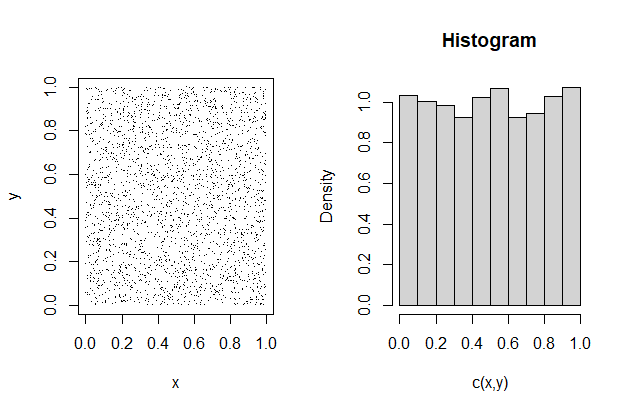
\includegraphics[width =1\textwidth]{figure_man/random.png}
\end{center}

%<<eval=FALSE, include=FALSE>>=
%library("random")
%x = randomNumbers(5000, min = 1, max = 1e+06, col = 2) / 1e+06
%summary(x)
%@
%<<echo=FALSE,>>=
%x = load2("random.rda")
%# summary(x)
%@

%<<echo=FALSE>>=
%par(mfrow = c(1, 2))
%colnames(x) = c("x", "y")
%plot(x, pch = ".")
%hist(matrix(x, ncol = 1), freq = FALSE, main = "Histogram", xlab = "c(x,y)")
%@
\end{vbframe}

\begin{vbframe}{Pseudo-random Numbers}
\begin{itemize}
 %\item \enquote{Random} source of random numbers, through simple recursive algorithm on the computer.
 \item \textbf{Definition}: A sequence of pseudo-random numbers is a
  deterministic (!) sequence of numbers with the same relevant
  properties as a sequence of independent and identically distributed
  random variables.
 \item Usually numbers from discrete and continuous uniform distributions,
  other distributions result from transformations.
 \item Starting point: Let $x_i$ be a sequence of natural numbers with discrete uniform distribution on the
  interval $[0,m]$. Then $u_i=x_i/m$ (with $m$ being large) is an approximation of the continuous uniform distribution with numerical precision $1/m$.
\end{itemize}


\framebreak

\begin{description}
 \item[Initial value $x_0$:] Must be specified, initialization is frequently done based on the system time. \enquote{Random} experiments with
  \textbf{Pseudo-random number generators (PRNG)} can be reproduced completely
  if the initial value is known (\enquote{seed value}).
 \item[Period:] Since there is only a finite set of numbers available, at some point $x_k=x_0$ must hold and the sequence repeats itself: $x_{i+k}=x_i$, $x_{i+k+1}=x_{i+1}$, \ldots
\end{description}

\lz

PRNG with periods as long as possible are desirable.

\end{vbframe}


%\section{Uniform distribution}

\begin{vbframe}{Quality criteria for PRNG}
Relevant properties of PRNG for uniformly distributed random numbers on $(0, 1)$:
\begin{itemize}
\item Actual uniform distribution on $(0, 1)$.
\item Distributions of pairs, triplets, etc. are also random (especially for multidimensional
  uniform distribution).
\item Period length. If the period is too short, then \ldots
\begin{itemize}
\item \ldots many integers cannot be realized (problem due to uniform distribution)
\item \ldots there are not enough independent random numbers
\end{itemize}
\end{itemize}
The \emph{relevance of each property} depends very much on the respective
application.
\end{vbframe}

\begin{vbframe}{Testing PRNG}
In order to assess the quality of PRNGs, they are subject to strict random number test suites.
The best known is \enquote{Die Hard} from George
Marsaglia (available for free):
\begin{itemize}
 \item Considered individually, is each bit i.i.d.\ 0 or 1 with probability $1/2$?
 \item Spectral test: Are $n$-tuples uniformly distributed in the unit cube?
  Are there autocorrelations?
 \item Rank of binary $6\times 8$ and $32\times 32$ matrices.
 \item \proglang{R} package \pkg{RDieHarder} \\
    \url{http://cran.r-project.org/web/packages/RDieHarder/}
\end{itemize}
\end{vbframe}


\endlecture

\end{document}